\begin{figure}[H]
    \begin{center}
    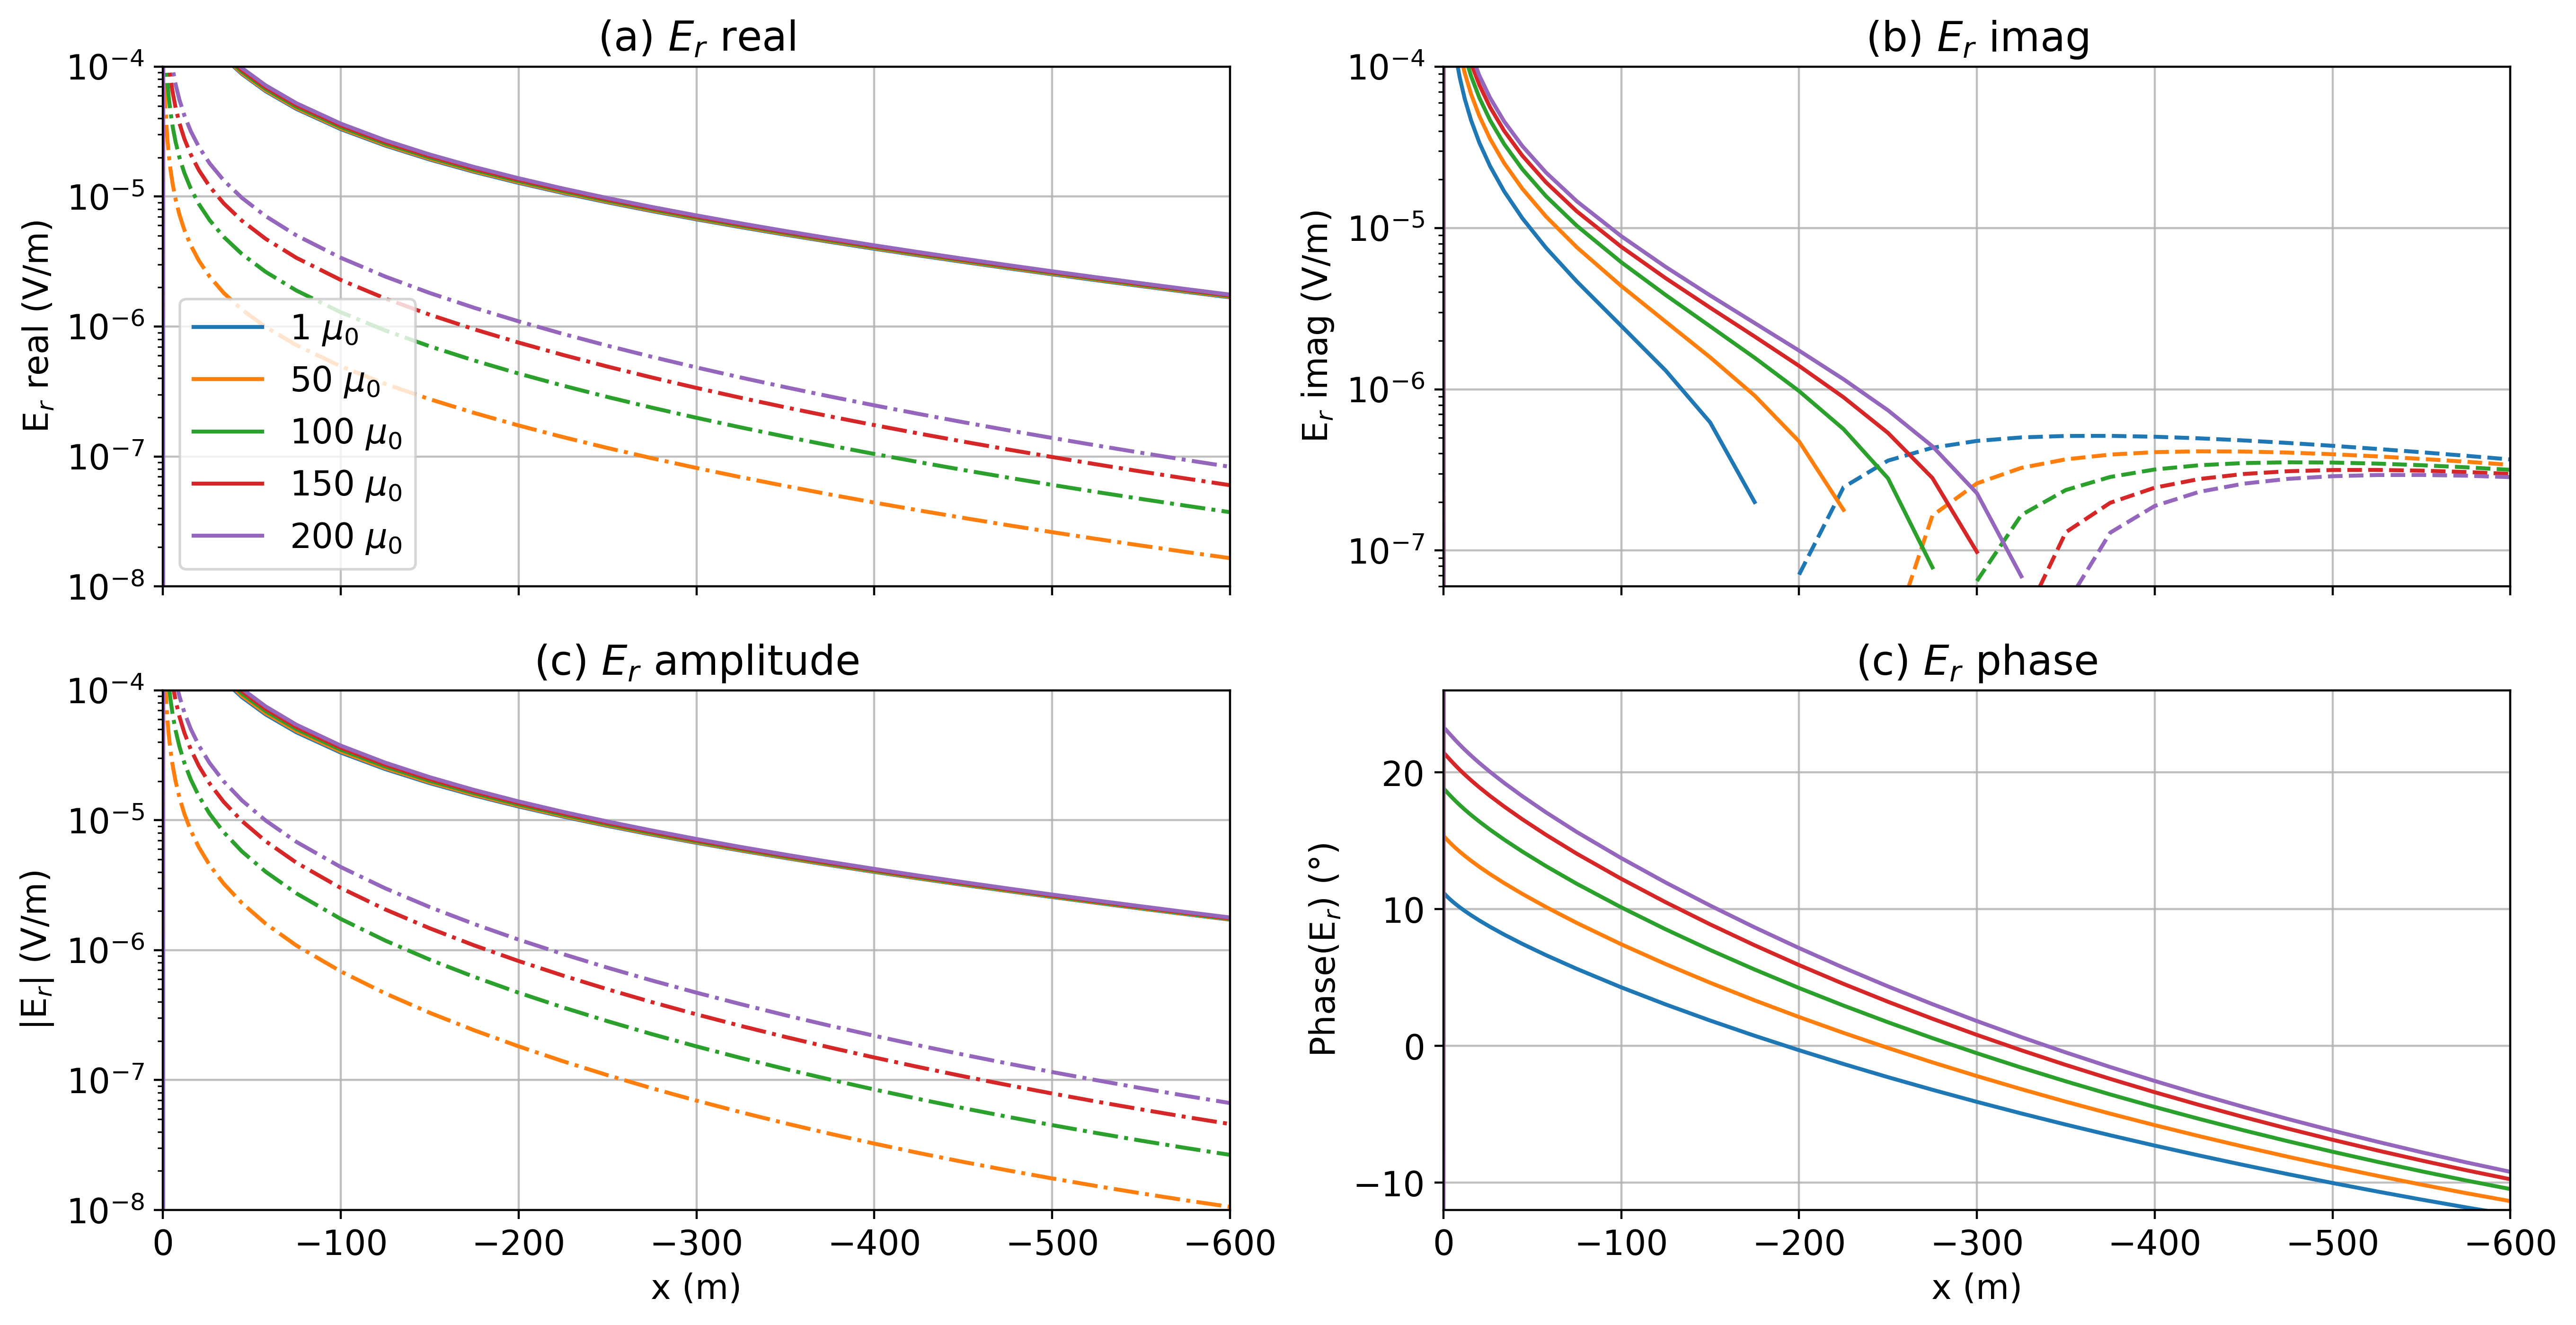
\includegraphics[width=\columnwidth]{figures/e-fields-fdem.png}
    \end{center}
\caption{
    Radial electric field data for a top-casing experiment at 5Hz: (a) real, (b) imaginary, (c) amplitude, and (d) phase. Solid lines indicate positive values and dashed lines indicate negative values. In (a) and (c) the difference between the permeable well scenarios and a non-permeable well ($\mu_r=1$) is shown with the dash-dot lines.
}
\label{fig:e-fields-fdem}
\end{figure}



